%%%%%%%%%%%%%%%%%%%%%%%%%%%%%%%%%%%%%%%%%%%%%%%%%%%%%%%%%%%%%%%%%%%%%%%%%%
%
% StEvent - User Guide and Reference Manual -- LaTeX Source
%
% $Id: StEstMaker.tex,v 1.1 2000/12/07 11:14:33 lmartin Exp $
%
% Author: Thomas Ullrich, March 1999
%
%%%%%%%%%%%%%%%%%%%%%%%%%%%%%%%%%%%%%%%%%%%%%%%%%%%%%%%%%%%%%%%%%%%%%%%%%%
%
% Notes to the authors:
%
% - A template for a class reference is at the end of this file.
% - Wrap all names functions with \name{}
% - All code, examples, prototypes in \verb+ ... +\\
%   or /begin{verbatim} ... \end{verbatim}
% - Use \StEvent if you refer to the package itself (not the class)
%
% This file is best edit with xemacs and the 'Function' package loaded.
%
%%%%%%%%%%%%%%%%%%%%%%%%%%%%%%%%%%%%%%%%%%%%%%%%%%%%%%%%%%%%%%%%%%%%%%%%%%
% Revision 1.1  1999/03/09 17:28:28  ullrich
% Initial Revision
%
%%%%%%%%%%%%%%%%%%%%%%%%%%%%%%%%%%%%%%%%%%%%%%%%%%%%%%%%%%%%%%%%%%%%%%%%%%
\documentclass[twoside]{article}

\parindent 0pt
\parskip 6pt
\advance\textwidth by 80pt%
\advance\evensidemargin by -80pt%

\usepackage{graphicx}
\usepackage{psboxit}
\usepackage{amsmath}
\usepackage{amssymb}
\usepackage{amsfonts}
\usepackage{fancyhdr}
\usepackage{times}
\usepackage{verbatim}
\usepackage{makeidx}
\usepackage{multicol}

\PScommands      % init boxit
\makeindex

%%%%%%%%%%%%%%%%%%%%%%%%%%%%%%%%%%%%%%%%%%%%%%%%%%%%%%%%%%%%%%%%%%%%
%
% Define header and footer style
%
%%%%%%%%%%%%%%%%%%%%%%%%%%%%%%%%%%%%%%%%%%%%%%%%%%%%%%%%%%%%%%%%%%%%
\pagestyle{fancyplain}
\rhead[\fancyplain{}{\bfseries\leftmark}]
      {\fancyplain{}{\bfseries\rightmark}}
\lhead[\fancyplain{}{\bfseries\rightmark}]
      {\fancyplain{}{\bfseries\leftmark}}
\rfoot[{}]{\fancyplain{}{\bfseries\thepage}}
\lfoot[\fancyplain{}{\bfseries\thepage}]{}
\cfoot{}

%%%%%%%%%%%%%%%%%%%%%%%%%%%%%%%%%%%%%%%%%%%%%%%%%%%%%%%%%%%%%%%%%%%%
%
% Typographic Conventions
%
%%%%%%%%%%%%%%%%%%%%%%%%%%%%%%%%%%%%%%%%%%%%%%%%%%%%%%%%%%%%%%%%%%%%
\newcommand{\name}[1]{\textsl{#1}}%  class-, function-, package names
\newcommand{\StestMaker}{\textsf{StEstMaker}}

%%%%%%%%%%%%%%%%%%%%%%%%%%%%%%%%%%%%%%%%%%%%%%%%%%%%%%%%%%%%%%%%%%%%
%
% Define multi line labels for class reference
%
%%%%%%%%%%%%%%%%%%%%%%%%%%%%%%%%%%%%%%%%%%%%%%%%%%%%%%%%%%%%%%%%%%%%
\newcommand{\entrylabel}[1]{\mbox{\textbf{{#1}}}\hfil}%
\newenvironment{entry}
{\begin{list}{}%
    {\renewcommand{\makelabel}{\entrylabel}%
     \setlength{\labelwidth}{90pt}%
     \setlength{\leftmargin}{\labelwidth}
     \advance\leftmargin by \labelsep%
      }%
    }%
  {\end{list}}

\newcommand{\Entrylabel}[1]%
{\raisebox{0pt}[1ex][0pt]{\makebox[\labelwidth][l]%
    {\parbox[t]{\labelwidth}{\hspace{0pt}\textbf{{#1}}}}}}
\newenvironment{Entry}%
{\renewcommand{\entrylabel}{\Entrylabel}\begin{entry}}%
  {\end{entry}}

\begin{document}

%%%%%%%%%%%%%%%%%%%%%%%%%%%%%%%%%%%%%%%%%%%%%%%%%%%%%%%%%%%%%%%%%%%%
%
%    Title page
%
%%%%%%%%%%%%%%%%%%%%%%%%%%%%%%%%%%%%%%%%%%%%%%%%%%%%%%%%%%%%%%%%%%%%
\begin{titlepage}
\pagestyle{empty}
\vspace*{-35mm}
\begin{center}
  \mbox{
\includegraphics[width=2cm]{StarIcon.eps}}
  {\Large\bf STAR Offline Library Long Writeup}
  \hfill\mbox{}\\[3cm]
  \mbox{\includegraphics[width=\textwidth]{StEstMakerTitle.eps}}
  \hfill\mbox{}\\[3cm]
  {\LARGE User Guide and Reference Manual}\\[2cm]
  {\LARGE $ $Revision: 1.1 $ $}  \\[5mm] % replaced by cvs with current revision
  {\LARGE $ $Date: 2000/12/07 11:14:33 $ $}  % replaced by cvs with current revision
  \vfill
\end{center}
\cleardoublepage
\end{titlepage}
\pagenumbering{roman}

%%%%%%%%%%%%%%%%%%%%%%%%%%%%%%%%%%%%%%%%%%%%%%%%%%%%%%%%%%%%%%%%%%%%
%
%    Table of content
%
%%%%%%%%%%%%%%%%%%%%%%%%%%%%%%%%%%%%%%%%%%%%%%%%%%%%%%%%%%%%%%%%%%%%
\tableofcontents
\cleardoublepage

%%%%%%%%%%%%%%%%%%%%%%%%%%%%%%%%%%%%%%%%%%%%%%%%%%%%%%%%%%%%%%%%%%%%
%
%    User Guide
%
%%%%%%%%%%%%%%%%%%%%%%%%%%%%%%%%%%%%%%%%%%%%%%%%%%%%%%%%%%%%%%%%%%%%
\pagenumbering{arabic}
\part{User Guide}
%%\clearpage

%%%%%%%%%%%%%%%%%%%%%%%%%%%%%%%%%%%%%%%%%%%%%%%%%%%%%%%%%%%%%%%%%%%%

\section{Introduction}
Quite a long time ago, two tracking methods have been developed to
perform independent track reconstruction in the SVT. The so-called
grouper or SGR
\footnote{See for details : STAR Note \#0153 or 
http://www.star.bnl.gov/STAR/html/svt\_{}l/soft\_{}l/svt\_{}software/sgr/SvtSgr.html}
is using a global mapping technique to group SVT hits into segments of
three hits. Since the method assumes that tracks come the main vertex,
the grouper is quite efficient in finding primary tracks. The second
method STK\footnote{See for details : STAR Note \#0145 or
http://www.star.bnl.gov/STAR/html/svt\_{}l/soft\_{}l/svt\_{}software/stk/SvtStk.html}
is reconstructing SVT tracks using a follow your nose technique.  STK
is generally used after a first pass using SGR and in a mode devoted
to the reconstruction of secondary particles. Once the three hit
segments are formed in the SVT, an other method SVM\footnote{See for details :
http://www.star.bnl.gov/STAR/html/svt\_{}l/soft\_{}l/svt\_{}software/svm/SvtSvm.html}

 is used to try to
associate them individually to the tracks reconstructed in the TPC.

The Silicon Strip Detector (SSD) is an additional layer which will be
install in between the outermost layer of the SVT and the inner radius
of the TPC. Two main advantages were foreseen when proposing the SSD
to enhance the STAR tracking capabilities : to add an extra hit to
each track passing through the SVT and recover the tracks lost due to
geometrical inneficiency, to extend the short lived particle
acceptance by reconstructing the track of daughter particles produced
at a radius bigger than the innermost SVT layer. Several attempts have
been made in order to extend the SVT tracking methods to include the
SSD. Performances obtained with STK adapted to a four layer geometry
were quite poor especially for secondary tracks for which the impact
of the SSD is supposed to be the more important. 
 
In order to fully benefit from the SSD a new tracking method called
EST has been developed. The main idea of the method is to start from
the reconstructed TPC tracks and to iteratively try to associate hits
from the SSD and the SVT layers. The method allows to find a priori
with the same efficiency primary and secondary tracks since no main
vertex constrain is imposed. Moreover, no lower limit being set on the
number of hits forming the segments in the vertex detector, the method
does not preclude the reconstruction of daughter tracks coming from
short-lived particle decaying far from the main vertex. In order to
maximize the efficiency of the method, the easiest tracks to find are
searched first : the tracks with the higher momentum and the tracks
leaving 4 hits in the vertex detector (by requiring four hits to be
associated during the first steps).

This method has been implemented and used to demonstrate the impact of
the SSD on the STAR capabilities\footnote{See for details : STAR Note
\#0400}. Whereas the obtained performances were quite good, simple 
modifications of the method were foreseen in order to improve these
results. The original version of the code was written in FORTRAN and
in a form which did not allow a strait forward implementation of these
new ideas. Consequently a new version of EST has been written in C++
which includes the improvement of the method. This document is
referring to this version of the method. Following this introduction,
the first main part of this manual contains a presentation of the
method and the code organization followed by some results illustrating
the performances obtained with EST. The second part of the document is
devoted to a more detailed description of the main objects and
methods implemented in the code completed by a full description of the
classes developed in the code.


%%%%%%%%%%%%%%%%%%%%%%%%%%%%%%%%%%%%%%%%%%%%%%%%%%%%%%%%%%%%%%%%%%%%

\section{Description of the tracking method}
\label{sec:Principles}

\subsection{The main ingredients of the method}

As already mentioned above, the basic idea of this method is to
reconstruct the particle trajectories by doing track to hit
associations. Since the track reconstruction is done in the TPC in a
first stage, the parameters of the track (assumed to be perfect
helices) reconstructed in the TPC are known. From these parameters,
fro each track a prediction is done on the intercept of the track with
the SSD layer. If a hit in the SSD satisfies some geometrical
criteria, it is attached to the track. The track parameters are then
updated and a new prediction is made for the next outermost layer of
the silicon detector. These steps are repeated for the other layers
until the first SVT layer. If in a given layer, no hit satisfies the
association criteria, the track parameters are not updated and a
prediction is calculated for the next layer. 

New features have been added to the method which are illustrated on
the figure \ref{fig:idea}.Contrary to the original version of the
code, in a given layer several hits can be attached to the same track
which results in the formation of branches for the track. These
branches are extended in parallel to the first SVT layer at which
point a choice has to be made to decide which branch to finally
keep. This idea is based on two observations :
\begin{itemize}
\item quite often the correct hit to be associated to a track is not
the nearest to the track projection. This is especially true when
projecting the track on the SSD. Allowing only one branch to be formed
per track would strongly compromise the chances to correctly
associated the hits to those tracks.
\item usually a wrong hit association in a given layer strongly reduces 
the chance to prolongate this branches in the innermost layers. Thanks
to the good position resolution in the silicon wafers, the update of
the track parameters with a hit associated significantly improves the
quality of the projection in the next layer. Once again this is
especially true in the SSD layer. This allows us to use stronger
geometrical criteria for the innermost layers and leads to prediction
for the wrong branch in an area where no hit satisfy these criteria.
\end{itemize}

\begin{figure}[h]
    \begin{center} 
	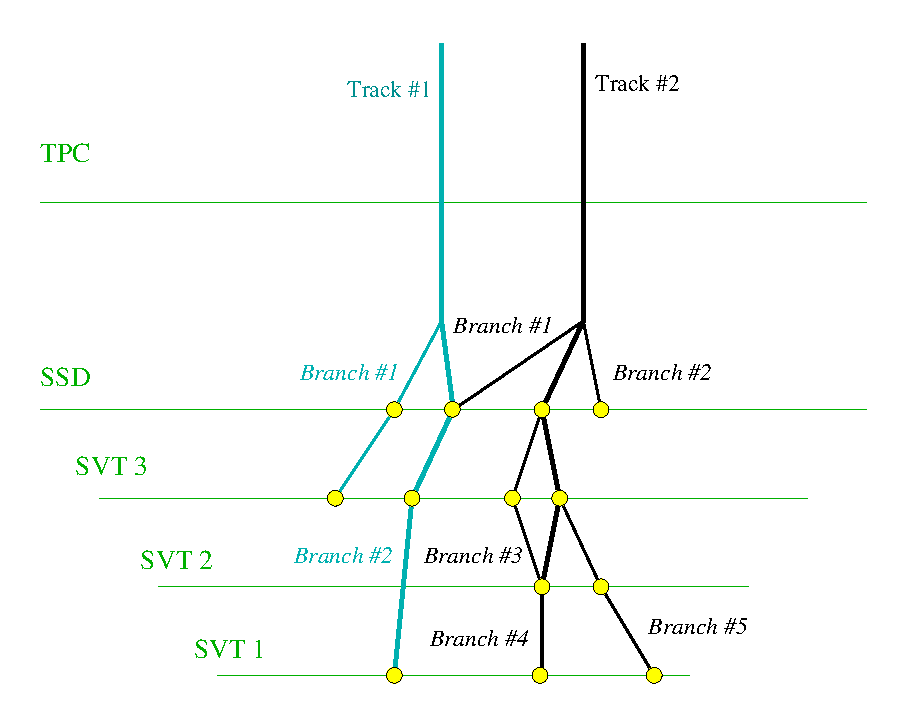
\includegraphics[width=0.8\textwidth]{idea.eps}
    	\caption{Illustration of the track branching and hit sharing
    implemented in the new version of the code. Several branches can
    be formed for each track (2 branches for the Track \#1 and 5
    branches for the Track \#2). Hits are shared between branches (the
    first hit from the left of the second SVT layer) and between
    tracks (the second SSD hit from the left).\label{fig:idea}} 
\end{center}
	
\end{figure}

An other new improvement which is used a combine manner with the track
branching is the possibility to allow hit sharing for tracks (the
sharing of the hits by different branches belonging to the same track
is implicitly implemented in the branching method). In a similar
fashion of the excluding the track branching, without hit sharing
between tracks, a incorrect hit to track association would ruin the
chances to associate a given hit to its correct track. 

After an detailed analysis of the quality of the tracks sharing one
or several hits, one can found out that most of the time the chi
square (of the refitted track) of the wrong tracks is higher than the
one of the correct one.  As a consequence at a given stage of the
tracking phase, the hit sharing is suppressed. More precisely, the hit
shared by several tracks are identified then all the tracks using a
given hit are sorted by increasing chi square. The track with the
lowest value is kept whereas the other tracks are deleted and their
hits (including those which are not shared) released for future
associations.

The hit to track association in consecutive layers is the basic step
used in the tracking part of EST. In order to maximize the tracking
performances, this step is applied successively to several defined
samples of tracks. This iterative procedure is motivated by the
obvious idea of first searching the tracks which are supposed to be
the easiest to find. The contribution of the multiple scattering
increasing with a decreasing momentum leads us to starts with the
tracks with the highest momentum. The iterative search is thus
organized into passes. Each passe is dedicated to the tracking of
tracks with a transverse momentum within a given range.

Taking into account the geometrical unefficiency, the slightly
different rapidity coverage of the layers, the main vertex spread
along the beam axis and the radial distribution of the secondary
vertices, one should expect to look for tracks with various patterns
and sizes for the hit segments in the vertex detector. Although, the
tracking method is required to be able to reconstruct all these kind
of tracks, is seems reasonable to iteratively search for a given type
at a time. As already stated, the association of a hit in a given
layer strongly constrains the possible associations in the inner
layers. This idea is implemented in the code by the mean of
superpasses. In the first superpass, one requires that the branch
formed possess a hit in all the active layers. During the last
superpass, loose cuts are applied and can be for example devoted to
the search of one hit segment without a specific location required for
this hit.

The various passes dedicated to the search of tracks with a given
transverse momentum are integrated into the superpass iterations. At
the end of a given pass, a unique branch is selected for each track
considered during this pass using the branch chi squares and hit
pattern and segment size requirements set for the current superpass.
More precisly, those requirements are not applied once all the
branches are completly formed but during the branch formation time
(ie. during the loops over the layer). After the tracking in a given
layer, knowing the hits already attached and the remaining layers to
scan, the branches which have no chances to fulfill the superpass
requirements are supressed. This particular location of the segment
selection in the tracking steps is improving the cpu time consumption
but more importantly maximize the chances to form branches with the
correct pattern.

Finally, the last new feature which has been introduced in the new
version of this method is the possibility to use information on the
main vertex location in order to improve the accuracy of the
predictions when projecting the tracks on the vertex detector layers.
The main vertex location is used as a guide to give an improved
prediction when trying to associate the first hit to the tracks. In
the current impementation the main vertex information can be used only
for tracks which already point toward it (using a initial distance of
closest approach to it) or for the full sample of tracks. Morever once
a first hit association has been done, it can be removed when updating
the track parameters or kept until the end of the branch formation
phase.

\subsection{Current implementation of the method}

To be done...

%%%%%%%%%%%%%%%%%%%%%%%%%%%%%%%%%%%%%%%%%%%%%%%%%%%%%%%%%%%%%%%%%%%%


\section{Performances}
\label{sec:performances}

\subsection{Track projection accuracy versus the primary vertex}
\subsection{Efficiency vs hit sharing}
\subsection{Efficiency vs track branching}
\subsection{General performances for the full tracking steps}
\subsection{Detailled analysis of the performances}

%%%%%%%%%%%%%%%%%%%%%%%%%%%%%%%%%%%%%%%%%%%%%%%%%%%%%%%%%%%%%%%%%%%%


\section{Current code limitations and future improvements}
\label{sec:limitations}

\clearpage

%%%%%%%%%%%%%%%%%%%%%%%%%%%%%%%%%%%%%%%%%%%%%%%%%%%%%%%%%%%%%%%%%%%%
%
%    Reference Manual
%
%%%%%%%%%%%%%%%%%%%%%%%%%%%%%%%%%%%%%%%%%%%%%%%%%%%%%%%%%%%%%%%%%%%%
\part{Reference Manual}
%%\clearpage

%%%%%%%%%%%%%%%%%%%%%%%%%%%%%%%%%%%%%%%%%%%%%%%%%%%%%%%%%%%%%%%%%%%%
\section{Description of the main objects and methods}
\subsection{StEstMaker}
\index{StEstMaker|textbf}
\label{sec:StEstMakerq}
%%%%%%%%%%%%%%%%%%%%%%%%%%%%%%%% mParams
\subsubsection{mParams}
\index{mParams|textbf}
\label{sec:mParamsq}
The \verb+mParams+ objects contain the parameters which are set for
each pass over pt. The key parameters stored in these objects are :
\begin{itemize}
\item \verb+onoff[i]+ : Determines if the layer i (0 to 2 are the SVT 
layers and 3 is the SSD) is active or not. By setting \verb+onoff[3]+
to 0 allow to switch from a year-3 to a year-2 geometry.
\item \verb+nbranch[i]+ : Sets to the allowed number of branches which can 
be formed in a given layer i. It corresponds to the number of new
branches allowed to be formed in a layer per mother branch
constructed in the previous layer or from the TPC tracks in the case
of the SSD layer.\\ By setting all the \verb+nbranch+ to 1, the
branching is forbitten in the pass.
\item \verb+ntotbranch[i]+ : Sets the maximum number of branches 
per track kept after the tracking in a given layer. The combination of
the \verb+nbranch+ parameters can lead to a value bigger than
\verb+ntotbranch+. The ChooseBestNBranches method limits the number of
branches to \verb+ntotbranch+ by selecting those with the lower
chisquares after re-fitting.
\item \verb+share[i]+ : Determines the number of times that a hit can 
be shared by different tracks. There is no limit on the number of
branches from the same track which can share a given hit.
\item \verb+geomcutl[4]+ and \verb+geomcutw[4]+ : Set the upper limits 
on the distance along the z axis and in the x-y plane between the
branch projection and the candidate hits.
\end{itemize}

The optimization of the tracking performances in term of efficiency
and purity is a balance between these parameters. Values bigger than
one for the branching and sharing parameters tends to support the
correct association although the correct hits are not at the first
rank in term of distances. The ranking of the correct association can
be checked using the root histograms named ``LocationX'' where X is a
layer index and built during the tracking phase.

On the other hand, the parameters controlling the geometrical cuts in
each layer tend to limit the number of hit candidates which can be
associated to a given branch in a given layer. Setting those cuts to a
large value is not reasonable since the number of wrong branches will
strongly increase and affect the efficiency of the branch selection
performed later on. They have to be set by knowing the accuracy of the
projection one can expect in a given layer and taking into account the
hits already attached from the previous layers. Several root
histograms are filled named ``disthitipX'',''disthitipXl'' and
``disthitipXw'' repectively filled with the hit-projection 3d
distances, distances along the z axis and distances in the transverse
plane assuming a perfect tracking. 

The histograms mentionned above are currently filled for the tracks
having 4 hit segment and in a year-3 geometry. They can be easily
adapted for various type of segments.


\begin{table}[ht]
\begin{center}
\begin{tabular}{|c|c|c|}\hline
Pass & ptmax & ptmin \\ \hline 
0 & 100. & 1.0 \\ \hline 
1 & 1.0 & 0.7
\\ \hline 
2 & 0.7 & 0.4 \\ \hline 
3 & 0.4 & 0.2 \\ \hline 
4 & 0.2 & 0.1 \\ \hline
\end{tabular}
\end{center}
\label{tab:passes_pt}
\caption{Upper and lower limits in transverse momemtum for the passes}
\end{table}

\begin{table}[ht]
\begin{center}
\begin{tabular}{|c|c|c|c|c|}\hline
Pass & cutl[3] & cutl[2] & cutl[1] & cutl[0] 
\\ \hline 
0 & 1.0 & 0.5 & 0.2 & 0.2 \\ \hline 
1 & 1.0 & 0.5 & 0.2 & 0.2 \\ \hline 
2 & 1.5 & 0.5 & 0.2 & 0.2 \\ \hline 
3 & 3.0 & 0.5 & 0.2 & 0.2 \\ \hline 
4 & 5.0 & 0.5 & 0.2 & 0.2 \\ \hline
\end{tabular}
\end{center}
\caption{Geometrical cuts along the beam axis for five passes and the four layers.}
\label{tab:geo}
\end{table}

\begin{table}[h]
\begin{center}
\begin{tabular}{|c|c|c|c|c|}\hline
Layer & onoff & share & nbranch & ntotbranch 
\\ \hline 
0 & 1 & 5 & 1 & 6 \\ \hline 
1 & 1 & 5 & 1 & 6 \\ \hline 
2 & 1 & 5 & 2 & 6 \\ \hline 
3 & 1 & 5 & 3 & 6 \\ \hline 
\end{tabular}
\end{center}
\caption{Track branching and hit sharing parameters for a given pass and the four layers}
\label{tab:bra}
\end{table}

Currently 5 passes are defined with the \verb+ptmin+ and
\verb+ptmax+ values (in GeV/c) summarised in the table~\ref{tab:passes_pt}.
As an example, the tables \ref{tab:geo} and \ref{tab:bra} contains the
parameter values currently used in a superpass which looks for 4 hit
segments. The geometrical cuts in the transverse plane are equal to
those in along the z axis. One can observe that the cuts in the SSD
are increasing with the pass number in order to compensate for the
decreasing accuracy of the TPC track projection. Morever the cut
values decrease when going from the SSD to the innermost SVT layer
which relies on the expected improvement of the track projection
accuracy when attaching more hits to the tracks. Based on the same
expectation the branching in the SSD is set to 3 while on the
innermost layers only 1 branch is allowed.


%%%%%%%%%%%%%%%%%%%%%%%%%%%%%%%% mSegments
\subsubsection{mSegments}
\index{mSegments|textbf}
\label{sec:mSegmentsq}
The \verb+mSegments+ parameters allow to set and control the
requirements for each super-pass. Two types of parameters are stored
in these objects which are respectively related to the caracteristics
of the TPC tracks that one tries to prolongate and to the hit pattern
of the segments which are formed during the super-passes.

Some of the TPC tracks are excluded for the tracking using the
parameters \verb+minTPChits+ which set a lower limit on the number of
hits in the TPC attached to the track and the parameters
\verb+rminTPC+ which set a upper limit on the distance in the 
transverse plane between the STAR geometrical center and the first TPC
hit. These parameters allow to temporarily flag the short TPC tracks
and the TPC tracks reconstructed in the outer part of the TPC for
which a relatively poor prediction of the track projection is expected.
These parameters are used in the \verb+FlagTPCTracksSP+ method 
(see \ref{sec:FlagTPCTracksSPq}).\index{FlagTPCTracksSP|textbf}


The hit pattern criteria for the segments formed during a given
super-pass are determined by the \verb+minhits+ parameter which sets a
lower limit on the number of SVT/SSD hits and the /verb+slay[i]+
parameters. In a given layer \verb+i+ the association of a hit to a
track can be forbidden \verb+slay[i]=0+, allowed \verb+slay[i]=1+ or
required \verb+slay[i]=2+. The table \ref{tab:seg} shows three
examples of settings for these parameters. The \verb+ChooseSegment+ 
\index{ChooseSegment|textbf} method uses these parameters to select
branches formed during the tracking phase.

\begin{table}[h]
\begin{center}
\begin{tabular}{|c|c|c|c|}\hline
 & A & B & C\\ \hline 
slay[0] & 2 & 1 & 1\\ \hline 
slay[1] & 2 & 1 & 1\\ \hline 
slay[2] & 2 & 1 & 1\\ \hline 
slay[3] & 2 & 2 & 1\\ \hline 
minhits & 4 & 3 & 1\\ \hline 
\end{tabular}
\end{center}
\caption{Examples of segment criteria: In the case A four hits are required 
with obviously a hit in every layer; in the case B a minimun number of
three hits are requiered with a mandatory hit in the SSD; in the case
C at least one hit is required without any specific layer origin.}
\label{tab:seg}
\end{table}

The last parameter \verb+chisqcut+ of the \verb+mSegment+ object can
be set to impose a higher limit on the chisq value of the fitted
branches.  This parameter is not used at this moment but can be easily
implemented in the \verb+ChooseBestNBranches+ 
\index{ChooseBestNBranches|textbf} and \verb+ChooseBestBranch+ 
\index{ChooseBestBranch|textbf} for instance.

%%%%%%%%%%%%%%%%%%%%%%%%%%%%%%%% Preprojection
\subsubsection{Preprojection}
\index{Preprojection|textbf}
\label{sec:Preprojectionq}
The aim of this method is to quickly determine for each branch formed
by the tracker which wafers should be considered as containing
possible hit candidates to be associated to the branch.

The closest intercept of the helix track with a cylinder of radius
equal to the current layer radius is determined. The
(\verb+phi+,\verb+z+) position of the intercept is then compared with
the wafer map \verb+mIndexGeom+ \index{mIndexGeom|textbf}. The Wafers
in the corresponding (\verb+phi+,\verb+z+) cell are stored in the
\verb+mPreProjTable+\index{mPreProjTable|textbf}. This list of wafer 
to be scanned is then completed by considering the neighbors of the
wafers already in the list. The \verb+mPreprojNumber+ data member
contains the final number of wafers in the list.

The variable mPreprojection is locally used to avoid double counting
the wafers. The size of the output table \verb+mPreProjTable+ is
limited to MAXFINDWAF\index{MAXFINDWAF|textbf} usually set to 70.

%%%%%%%%%%%%%%%%%%%%%%%%%%%%%%%% Projection
\subsubsection{Projection}
\index{Projection|textbf}
\label{sec:Projectionq}
This method is called immediately after the \verb+Preprojection+
method and thus applied to each branch.

For each wafer stored in \verb+mPreProjTable+
\index{mPreProjTable|textbf}, the intercept of the track helix with the wafer plane
is calculated. Every hit contained in the current wafer is scanned and
is added to a list if :
\begin{itemize}
\item the hit is available (\verb+GetFlag()>0+)\index{GetFlag|textbf},
\item the distances in z and in the bending plane between the hit and 
the track projection are smaller than \verb+mParams[mPass]->geomcutl[slay]+ and 
\verb+mParams[mPass]->geomcutw[slay]+ \index{mParams|textbf},
\item the number of hits already considered is smaller than \verb+MAXHITPROJ+
\index{MAXHITPROJ|textbf}
\end{itemize}

The list \verb+mProjOut+ \index{mProjOut|textbf}
containing the accepted hits (possibly from different wafers) 
is sorted by increasing 3D distance between the hit and the track projection.
The maximum number of hits in this list \verb+MAXHITPROJ+ is usually set to 400. 

%%%%%%%%%%%%%%%%%%%%%%%%%%%%%%%% Init
\subsubsection{Init}
\index{Init|textbf}
\label{sec:Initq}

%%%%%%%%%%%%%%%%%%%%%%%%%%%%%%%% SVTInit
\subsubsection{SVTInit}
\index{SVTInit|textbf}
\label{sec:SVTInitq}

%%%%%%%%%%%%%%%%%%%%%%%%%%%%%%%% TPCInit
\subsubsection{TPCInit}
\index{TPCInit|textbf}
\label{sec:TPCInitq}

This method is called by the \verb+Init+ \index{Init|textbf} method to
initialize the objects related to the TPC tracks. The
\verb+StEstTPCTrack+ objects and the \verb+mTPCTrack+ \index{mTPCTrack|textbf}
table pointing to these objects are built. The TPC tracks with a
negative flag are not loaded. The mTptIndex translation table from the
track id to its row in the \verb+mTPCTrack+ table is constructed. 

For each track declared in \verb+mTPCTrack+ its hit table \verb+mR+ is built.
After the hit table has been built, the hits are sorted according to increasing order.

%%%%%%%%%%%%%%%%%%%%%%%%%%%%%%%% FlagTPCTracksSP
\subsubsection{FlagTPCTracksSP}
\index{FlagTPCTracksSP|textbf}
\label{sec:FlagTPCTracksSPq}

This method is called at the beginning of each super-pass to flag
some of the TPC tracks (of type \verb+StEstTPCTrack+) which will not
be considered for tracking in that super-pass. Currently two types of
tracks are rejected by using this special flag :

\begin{itemize}
\item 	TPC tracks with a number of hits 
smaller than \verb+minTPChits+ (from \verb+mSegments+) have a  
\verb+mFlagSP+ sets to -1,
\item TPC tracks with a distance (in the x-y plane) from the detector 
center to the innermost hit bigger than \verb+rminTPC+ have a \verb+mFlagSP+ sets to -2.
\end{itemize}



%%%%%%%%%%%%%%%%%%%%%%%%%%%%%%%% ChooseSegment
\subsubsection{ChooseSegment}
\index{ChooseSegment|textbf}
\label{sec:ChooseSegmentq}

This method is called at each tracking step to prevent from building
branches which at the end of the loop on the layers will not satisfy
the pattern criteria required for the current super-pass. These
criteria are sets in the \verb+mSegments+ object
\index{mSegments|textbf} and combine the \verb+minhits+ and the
\verb+slay[nlay]+ conditions. Branches are deleted if :

\begin{itemize}
\item the number of already attached hits plus the number of layers which remain to be scanned is smaller than \verb+minhits+.
\item the condition \verb+slay[i]+=2 requiering a hit in the layer \verb+i+ already scanned is not fulfilled.
\end{itemize}

%%%%%%%%%%%%%%%%%%%%%%%%%%%%%%%% ChooseBestNBranches
\subsubsection{ChooseBestNBranches}
\index{ChooseBestNBranches|textbf}
\label{sec:ChooseBestNBranchesq}

This method is called at each tracking step to prevent from building a
too large number of branches for each track. For each track in a given
layer, its branches are sorted by increasing chisq. In order to
emphasise on the SVT/SSD hit contribution to the chisq, the chisq of
the track obtained only with the TPC hits is first subtracted to the
total chisq.

Once sorted, the \verb+mParams[mPass]->ntotbranch[slay]+ branches with
the best chisq are selected. The remaining branches are deleted.

%%%%%%%%%%%%%%%%%%%%%%%%%%%%%%%% ChooseBestBranch
\subsubsection{ChooseBestBranch}
\index{ChooseBestBranch|textbf}
\label{sec:ChooseBestBranchq}

This method is called for each pass at the end of the tracking in all
the layers in order to select for each track a unique branch. For the
time being, the branch with the smaller chisq is selected. No upper
limit on the chisq value is applied. 


%%%%%%%%%%%%%%%%%%%%%%%%%%%%%%%% RemoveHitSharing
\subsubsection{RemoveHitSharing}
\index{RemoveHitSharing|textbf}
\label{sec:RemoveHitSharingq}

Depending on the value of \verb+share[nlay]+ in the \verb+mParams+
structure, hit sharing can be allowed. Hit sharing is quite usefull in
order to preserve the chances for a hit which is already connected to
a wrong branch to be in parallele attached to the correct one. By
studying the chisq of the branches formed after a given pass which
share some hits with some other branches, one can find that frequently
the correct branch has the smallest chisq. In addition, in some cases
hits are shared by two wrong branches. This method has been developed
in order to supress the number of bad branches without affecting too
much the number of correct branches. The method is called at the end
of each pass and do the following operations :

\begin{itemize}
\item Loop in the the hit object list and look for hit shared (\verb+mNShare+),
\item For each shared hit, select the branch with the smallest chisq among all the branches sharing the current hit,
\item For all branches with bigger chisq,  detache all the  hits (including the one which are not shared). 
\end{itemize}

%%%%%%%%%%%%%%%%%%%%%%%%%%%%%%%% Eval
\subsubsection{Eval}
\index{Eval|textbf}
\label{sec:Evalq}

The tracking evaluation can be performed at a first level analysis
corresponding to the usual counting of possible/good/bad tracks.

Three track status are required to calculate the efficiency and purity
of the tracking procedure. 

{\bf the number of ideal tracks :} all ideal (possible) TPC tracks with at least hit in the SVT/SSD.

{\bf the number of good tracks :} all  tracks which have been 
reconstructed with correct hits.

{\bf the number of bad tracks :} all reconstructed tracks with at least 
one wrong hit. 

One should note that in this evaluation function, the definition of
the ideal tracks is somehow more severe than the above
definition. Tracks which are not considered (trackable) by the
tracking method are excluded. As an example, a tracking pass
requiering a hit in every layers will lead to exclude tracks with less
that 4 hits from the ideal track list.

The efficiency and purity are defined as follow :

$$ \mbox{Efficiency} = \frac{\mbox{good}}{\mbox{possible}} \qquad \mbox{Purity} = \frac{\mbox{good}}{\mbox{good} + \mbox{bad}}$$

A detailed analysis of the tracking evaluation can be also made in
order to take into account the fact that a given TPC track can be
splitted into several segments. The idea is to count the number of TPC
tracks according their \verb+mcid+ instead of their \verb+id+.  In
other words, and in the view of future physics analyses, each produced
particle should be counted once independently from the fact that the
TPC tracking can reconstruct a track in one or several
segments. Consequently, a TPC track formed with, for example 2
segments, will be counted once as a possible track. With the former
evaluation, 2 different \verb+id+ would have been assigned to the segments
and thus 2 possible tracks would have been counted .

\vspace*{0.4cm}
In summary, if several segments belonging to one TPC track are
correctly associated, only one association will be counted, the other
ones will be considered as ghosts. 

%On the other hand, if several
%segments of the same TPC track are badly associated, one has to count
%all these bad association since it is the only way to take into
%account rigorously the pollution that the algorithm introduces in the
%track reconstruction.


The efficiency and the purity are defined as :

$$ \mbox{Efficiency} = \frac{\mbox{correct}}{\mbox{input}} \qquad \mbox{Purity} = \frac{\mbox{found}}{\mbox{found}}$$

\vspace*{0.4cm}

The following example illustrates the two evaluation methods applied
to a TPC track splitted into two segments. The efficiency and purity
are expressed in pourcentage.

\begin{center}
\begin{tabular}{|c|c|c|c|c|c||c|c|c|c|c|} \hline
&\multicolumn{5}{|c||}{Detailled analysis}&\multicolumn{5}{|c|}{First Level analysis}\\ \hline
Association & Input & Found & Correct & Effi. & Purity & Possible & Good & Bad & Effi. & Purity \\ \hline
2 bad        & 1 & 2 & 0 &   0 &  0 & 2 & 0 & 2 &   0 &  0\\ \hline    
1 bad 1 good & 1 & 2 & 1 & 100 & 50 & 2 & 1 & 1 &  50 & 50\\ \hline    
2 good       & 1 & 2 & 1 & 100 & 50 & 2 & 2 & 0 & 100 &100\\ \hline    
1 good       & 1 & 1 & 1 & 100 &100 & 2 & 1 & 0 &  50 &100\\ \hline    
1 bad        & 1 & 1 & 0 &  0  &  0 & 2 & 0 & 1 &   0 &  0\\ \hline    
\end{tabular}
\end{center}

\vspace*{0.4cm}
Several classes of tracks are distinguished in the eval method and
output on the screen :

\vspace*{0.2cm}
\underline{Among all ideal tracks :} 

$\bullet$ Ideal not found but unique : ideal track not
reconstructed. Its mcid is unique, and not shared by an other TPC
segment.

$\bullet$ Ideal not found but copy in good : ideal track not reconstructed 
but with a copy (i.e. another TPC segment with the same mcid) which
has been correctly reconstructed.  

$\bullet$ Ideal not found but copy in bad : ideal track not reconstructed 
but with a copy which has been badly reconstructed.   

$\bullet$ Ideal not found but copy in ideal: ideal track not reconstructed and 
with a copy which is not reconstructed either.

$\Longrightarrow$ Real ideal tracks : all the ideal tracks minus all the 
possible copies. 

\vspace*{0.3cm}
\underline{Among all good tracks : }

$\bullet$ Good found twice in good : a track correctly reconstructed
but with a copy which is also correctly reconstructed. One of the 2
correct segments is considered as a bad track.

$\Longrightarrow$ Real good tracks : all the initial number of good tracks minus the
good tracks found twice.



\vspace*{0.3cm}
\underline{Among all bad tracks: }

$\bullet$ Bad in ideal : track badly reconstructed which is in the ideal track list.

$\bullet$ Bad not in ideal : track badly reconstructed and which was
not in the ideal set of tracks. They are for example the TPC tracks
which should not have any SVT/SSD hit attached.

$\bullet$ Bad found twice in bad : track badly reconstructed which has
already a copy in the bad track list.

$\Longrightarrow$ Real bad tracks : all the initial number of bad
tracks since it is used only in the purity estimate.

\section{Class Reference}
%%\clearpage

%%%%%%%%%%%%%%%%%%%%%%%%%%%%%%%%%%%%%%%%%%%%%%%%%%%%%%%%%%%%%%%%%%%%
%
%    Reference: StEstMaker
%
%%%%%%%%%%%%%%%%%%%%%%%%%%%%%%%%%%%%%%%%%%%%%%%%%%%%%%%%%%%%%%%%%%%%
\subsection{StEstMaker}
\index{StEstMaker|textbf}
\label{sec:StestMakerq}
\begin{Entry}
\item[Summary]

\item[Synopsis]
    \verb+#include "StEstMaker.hh"+\\ \verb+class StEstMaker;+\\

\item[Description]

\item[Persistence]
    None

\item[Related Classes]

\item[Protected Data\\ Member]
	\verb+St_DataSet* mEvent;+\\
	DataSet containing the EST output ??? \\
	\verb+St_DataSetIter* mEventIter;+\\
	Iterator on the Event DataSet.\\
	\verb+StEstWafer* mPreprojTable[MAXFINDWAF];+\\
	List of wafers build by the \verb+Preprojection+ method to be scanned by the \verb+Projection+ method.\\
	\verb+StEstParams** mParams;+\\
	Table containing the tracking parameters for the passes (over pt).\\
	\verb+StEstSegments** mSegments;+\\
	Table containing the tracking parameters for the superpasses (on the track pattern).\\
	\verb+StEstIndexGeom* mIndexGeom;+\\
	Coarse description of the SVT/SSD geometry.\\
	\verb+StEstWafer** mIndexWaf;+\\
	List of wafer objects.\\
	\verb+StEstHit** mSvtHit;+\\
	List of SVT/SSD hits.\\
	\verb+StEstHit* mVertex;+\\
	Main vertex.\\
	\verb+StEstTPCTrack**  mTPCTrack;+\\  
	List of TPC tracks (tracks with \verb+flag<0+ are not loaded).\\
	\verb+StEstTrack** mTrack;+\\
	List of global tracks.\\
	\verb+svg_shape_st* mSvgShape;+\\
	Table containing the SVT/SSD wafer shapes.\\
	\verb+StEstProjOut mProjOut;+\\ 
	List of candidate hits to be considered by the tracking.\\
	\verb+long* Eval_id_mctrk2est_Track;+\\
	To be explained.\\
	\verb+StEstHit*** Eval_mchits;+\\
	List of SVT/SSD hits for each tracks.\\
	\verb+long     mWafId2IndexWaf[9000];+\\
	Wafer id (1101,1102,..) to Wafer index (0,1,..) translation table.\\
	\verb+long* mTptIndex;+\\\
	Translation table between the TPC track id and its row number in the \verb+mTPCTrack+ table.\\
	\verb+long mNTPCTrack;+\\
	Number of TPC tracks (TPC tracks with negative flag are excluded).\\
	\verb+long mNTrack;+\\
	Number of global tracks.\\
	\verb+long mNSvtHit;+\\
	Number of SVT/SSD hits.\\
	\verb+int      mPass;+\\
	Current pass number.\\
	\verb+int      mNPass;+\\
	Number of passes.\\
	\verb+int      mSuperPass;+\\
	Current superpass number.\\
	\verb+int      mNSuperPass;+\\
	Number of superpasses.\\
	\verb+int      mStartLayer;+\\
	Index of the outermost layer used in the tracking.\\
	\verb+int      mEndLayer;+\\
	Index of the innermost layer used in the tracking.\\
	\verb+int      mPreprojNumber;+\\
	Number of wafers to be scanned by the \verb+Projection+ method.\\
	\verb+int      mIdealTracking;+\\
	Flag for the perfect tracking.\\
	\verb+long     mFindable;+\\
	Number of findable tracks.\\
	\verb+long     mFoundOK;+\\
	Number of good tracks found by the tracker.\\
	\verb+long     mFoundFake;+\\
	Number of ghost tracks generated by the tracker.\\
\item[Public\\ Constructors]
	\verb+StEstMaker(const char* name = "est");+\\
\item[Protected Functions]
	\verb+int  Preprojection(StEstBranch&, int);+\\
	Build a list of wafers to be scanned for a branch in a given layer.\\
	\verb+int  Projection(StEstBranch* branch, long slay);+\\
	Returns a list of hits which satisfy some distance criteria to the branch projection.\\
	\verb+int  Tracking(int);+\\
	Main tracking method.\\
	\verb+int  RefitBranch(StEstBranch *br, StEstHit* hit=NULL, int exclhit=-1, int usevertex=0);+\\
	Method used to refit the branch \verb+br+ with the additional hit \verb+hit+ possibly excluding some hits and using the main vertex.\\ 
	\verb+int SVTInit(St_DataSetIter* dataiter);+\\
	Initialises and fills the StEstWafer objects. \\
	Initialises and fills the StEstHit objects. \\
	\verb+int TPCInit(St_DataSetIter* dataiter);+\\
	Initialises and fills the StEstTPCTrack objects. \\
	\verb+void ChooseBestNBranches(StEstTrack *tr, int slay);+\\
	Choose a given number of branches after tracking in the layer \verb+slay+ for the track \verb+tr+.\\
\end{Entry}

%%%%%%%%%%%%%%%%%%%%%%%%%%%%%%%%%%%%%%%%%%%%%%%%%%%%%%%%%%%%%%%%%%%%
%
%    Reference: StEstParams
%
%%%%%%%%%%%%%%%%%%%%%%%%%%%%%%%%%%%%%%%%%%%%%%%%%%%%%%%%%%%%%%%%%%%%
\subsection{StEstParams}
\index{StEstParams|textbf}
\label{sec:StestParamsq}
\begin{Entry}
\item[Summary]
Structure containing the parameters for the passes.
\item[Public Data\\ Member]
\verb+int debug+;\\
Debugging level (0 = only critical errors are mentioned).\\
\verb+int onoff[4]+;\\
Tracking status for a given super-layer (1 = tracking is allowed for the 
considered layer; 0 = no tracking is performed within this layer).\\
\verb+double ptmin+;\\
Lowest pt value for a pass.\\
\verb+double ptmax+;\\
Maximum pt value for a pass.\\
\verb+int nbranch[4]+;\\
Number of daughter branches allowed to be formed in a layer per the
mother branch.\\
\verb+int ntotbranch[4]+;\\
Maximum number of branches per track kept after the tracking in a
given layer. 
\verb+int maxbranches+;\\
Maximum number of branches that can be attached to a track. This is
used temporarily to initialize the branch list of each Track to a
large value. Once the parameters \verb+nbranch+ and \verb+ntotbranch+
will be defined consistently, then \verb+maxbranches+ will become obsolete.\\
\verb+int share[4]+;\\
Number of times that a hit can be shared by different tracks.\\
\verb+int maxtpchits+;\\
Maximum number of hits per TPC track. It is used for the
initialization of the St\_TPCTrack object and corresponds to the
maximum number of TPC hits taken to this object.\\
\verb+int maxsvthits+;\\
Maximum number of SVT hits in the branches. It is used also to
initialize the size of the hit list of each branch. \\
\verb+double lrad[4][2]+;\\
Radii of the silicon detector layers. 2 values are set for the SVT layers (the sublayers)
and one for the SSD.\\
\verb+int nneighbours[4]+;\\
Number of rings of wafers which are neighbors of the wafer containing the track
projection and whose space points will be candidate for the track to
hit association.\\
\verb+double phibin+;\verb+double zbin+;\\
Size of the bins in phi and along the z direction.\\
\verb+int nphibin+;\verb+int nzbin+;\\
Number of bins in phi or z. \\ 
These last 4 parameters are used for
searching the \verb+nneighbourgs+ wafers. Since this step is performed
during the preprojection phase, they should be normally defined once,
and not like it is done now, for each pt pass.  \\
\verb+double geomcutl[4]+;\\
Geometrical cut for length (along z axis beam) used to define hit
searching areas.\\
\verb+double geomcutw[4]+;\\
Geometrical cut for width (in the x-y plane) used to define hit
searching areas.\\
\end{Entry}
%%%%%%%%%%%%%%%%%%%%%%%%%%%%%%%%%%%%%%%%%%%%%%%%%%%%%%%%%%%%%%%%%%%%
%
%    Reference: StEstSegment
%
%%%%%%%%%%%%%%%%%%%%%%%%%%%%%%%%%%%%%%%%%%%%%%%%%%%%%%%%%%%%%%%%%%%%
\subsection{StEstSegment}
\index{StEstSegment|textbf}
\label{sec:StestSegmentq}
\begin{Entry}
\item[Summary]
Structure containing the parameters for the super-passes.
\item[Public Data\\ Member]
\verb+int slay[nlay]+;\\
Hit requirements defined for each super-layer (2 = required; 1 =
allowed; 0 = forbidden).
\verb+int minhits+;\\
Minimum number of hits in a segment.\\
\verb+int minTPChits+;\\
Minimum number of hits that a TPC track has to contain for being
considered. \\
\verb+double rminTPC+;\\
Minimal radius at which the first hit (the nearest from the
geometrical center) of the TPC track has to be located. \\
\verb+double chisqut+; \\
Maximum allowed chisq value after the branch refitting (not used
anymore).\\
\end{Entry}
%%%%%%%%%%%%%%%%%%%%%%%%%%%%%%%%%%%%%%%%%%%%%%%%%%%%%%%%%%%%%%%%%%%%
%
%    Reference: StEstProjOut
%
%%%%%%%%%%%%%%%%%%%%%%%%%%%%%%%%%%%%%%%%%%%%%%%%%%%%%%%%%%%%%%%%%%%%
\subsection{StEstProjOut}
\index{StEstProjout|textbf}
\label{sec:StestProjOutq}
\begin{Entry}
\item[Summary]
Structure containing the output of the Projection Method for a given branch.
\item[Public Data\\ Member]
\verb+int nhit+; \\
Number of hits in hit array.\\
\verb+StEstHit* hit[MAXHITPROJ]+; \\
List of pointer to hits found in the projection.\\
\verb+double dist[MAXHITPROJ]+;\\
3D distance between the hit and the track projection.\\
\verb+double distw[MAXHITPROJ]+;\\
Distance in the transverse plane between the hit and the track projection.\\
\verb+double distl[MAXHITPROJ]+;\\
Distance along the z axis between the hit and the track projection.\\
\end{Entry}
%%%%%%%%%%%%%%%%%%%%%%%%%%%%%%%%%%%%%%%%%%%%%%%%%%%%%%%%%%%%%%%%%%%%
%
%    Reference: StEstGtrk
%
%%%%%%%%%%%%%%%%%%%%%%%%%%%%%%%%%%%%%%%%%%%%%%%%%%%%%%%%%%%%%%%%%%%%
\subsection{StEstGtrk}
\index{StEstGtrk|textbf}
\label{sec:StestGtrkq}
\begin{Entry}
\item[Summary]
Structure containing the inputs for the egr fitting routines.
\item[Public Data\\ Member]
\verb+long nhit+;\\
Number of hits in the track (SVT,SSD,TPC and main vertex).\\
\verb+long ipnt[220]+;\\
Pointers to the hits belonging to the track.\\
\verb+long pos[220];+;\\
Positions of the hits on the tracks.\\
\verb+long det[220];+;\\
Detector index of the hits (SVT/SSD,TPC,main vertex).\\
\verb+float p[9]+;\\ 
Track parameters output from the fitting routines.\\
\verb+long nfit+;\\
Number of hits included in the fit.\\
\verb+long flag+;\\
Status flag of the fit.\\
\verb+long ntpc+;\\
Number of hits belonging to the TPC.\\
\verb+long nmax+;\\
Maximum number of hits considered in the fit.\\
\end{Entry}
%%%%%%%%%%%%%%%%%%%%%%%%%%%%%%%%%%%%%%%%%%%%%%%%%%%%%%%%%%%%%%%%%%%%
%
%    Reference: StEstWafer
%
%%%%%%%%%%%%%%%%%%%%%%%%%%%%%%%%%%%%%%%%%%%%%%%%%%%%%%%%%%%%%%%%%%%%
\subsection{StEstWafer}
\index{StEstWafer|textbf}
\label{sec:StestWaferq}
\begin{Entry}
\item[Summary]
Class describing the SVT and SSD wafers.\\
\item[Synopsis]
    \verb+#include "StEstMaker.hh"+\\
    \verb+class StEstMaker;+\\
\item[Description]

\item[Persistence]
    None \\	

\item[Related Classes]
	
\item[Protected Data\\ Member]
    	\verb+int mShape;+\\
    	Geometrical shape of the wafer (taken from \verb+svg_geom.id_shape+).\\
	\verb+int mLayer;+\\
	Layer the wafer belong to. \\	
	\verb+long int mNHits;+\\
	Number of hits in the wafer. \\	
	\verb+long int mMaxHits;+\\
	Maximum number of hits in the wafer (usually 200).\\	
	\verb+StEstHit **mHits;+\\
	List of hits within the wafer. \\	
	\verb+StThreeVector<double>* x;+\\
	Position of the center of the wafer within the STAR global reference frame.\\ 	
	\verb+StThreeVector<double>* n;+\\
	Unitary vector normal to the wafer plane.\\
\item[Public Data\\ Member]
	\verb+char mPreprojection;+\\
	Flag for the preprojection method.\\
	\verb+long int mId;+\\
	Id of the wafer (according to the \verb+svg_geom+ table. Should be protected member\\
	\verb+StEstWafer* neighbour[8];+\\
	Table of neighbouring wafers.\\
\item[Public\\ Constructors]
	\verb+StEstWafer(long int nr, long int mh, StThreeVector<double>* xx,+\\ 
	\verb+StThreeVector<double>* nn, int shape);+\\

\item[Public Member\\ Functions]
	\verb+StThreeVector<double>* StEstWafer::GetX();+\\
	Returns the position of the center of the wafer.\\ 
	\verb+StThreeVector<double>* StEstWafer::GetN();+\\
	Returns the orientation vector of the wafer.\\
	\verb+StEstHit* GetHit(long nr);+\\
	Returns a pointer to the nr hit of the wafer.\\
	\verb+int AddHit(StEstHit *hit);+\\
	Adds a hit to the wafer hit list.\\
	\verb+int GetLayer();+\\
	Returns the wafer layer number.\\
	\verb+int GetShape();+\\
	Returns the wafer shape number.\\
	\verb+long GetNHits();+\\
	Returns the number of hits in the wafer.\\
	\verb+long int GetId();+\\
	Returns the id of the wafer.\\	
\end{Entry}

%%%%%%%%%%%%%%%%%%%%%%%%%%%%%%%%%%%%%%%%%%%%%%%%%%%%%%%%%%%%%%%%%%%%
%
%    Reference: StEstIndexGeom
%
%%%%%%%%%%%%%%%%%%%%%%%%%%%%%%%%%%%%%%%%%%%%%%%%%%%%%%%%%%%%%%%%%%%%
\subsection{StEstIndexGeom}
\index{StEstIdexGeom|textbf}
\label{sec:StestIndexGeomq}
\begin{Entry}
\item[Summary]
Class for the preprojection method.\\
\item[Synopsis]
    \verb+#include "StEstMaker.hh"+\\
    \verb+class StEstMaker;+\\
\item[Description]
	This class contains a simple SVT/SSD geometry description which allows a fast access to the wafer object located in a given z-phi area.\\
\item[Related Classes]
	
\item[Protected Data\\ Member]
	\verb+int*** nWaf;+\\
	Table containing the number of wafers per z bin and phi bin for each layer.\\	
	\verb+StEstWafer***** pWaf;+\\	
	Table pointing to the wafers in each bin in z and phi and in each layer.\\
	\verb+int nphibins;+\\
	Number of bins in phi to map the SVT/SSD geometry.\\
	\verb+int nzbins;+\\
	Number of bin in z to map the SVT/SSD geometry.\\
\item[Public Data\\ Member]
\item[Public\\ Constructors]
	\verb+StEstIndexGeom::StEstIndexGeom(int np, int nz)+\\
\item[Public Member\\ Functions]
	\verb+int setWafTab(int phi, int z, int slay, StEstWafer* waf)+\\
	Stores the wafer \verb+waf+ in the tables.\\
	\verb+int getNWaf(int phi, int z, int slay)+\\
	Returns the number of wafers in a given (z,phi) cell and a layer.\\
	\verb+StEstWafer** getWafTab(int phi, int z, int slay)+\\
	Returns a pointer list of the wafers contained in a given (z,phi) cell and a layer.\\
\end{Entry}

%%%%%%%%%%%%%%%%%%%%%%%%%%%%%%%%%%%%%%%%%%%%%%%%%%%%%%%%%%%%%%%%%%%%
%
%    Reference: StEstHit
%
%%%%%%%%%%%%%%%%%%%%%%%%%%%%%%%%%%%%%%%%%%%%%%%%%%%%%%%%%%%%%%%%%%%%
\subsection{StEstHit}
\index{StEstHit|textbf}
\label{sec:StestHitq}
\begin{Entry}
\item[Summary]
Class describing the SVT and SSD hits.\\
\item[Synopsis]
    \verb+#include "StEstBranch.hh"+\\
    \verb+class StEstWafer;+\\
    \verb+class StEstBranch;+\\
    \verb+class StEstMaker;+\\
\item[Description]

\item[Related Classes]
	
\item[Protected Data\\ Member]
	\verb+StEstWafer*   mDetector;+\\
	Id of the wafer containing the hit.\\
	\verb+StEstBranch** mBranch;+\\
	List of branches the hit is attached to.\\
	\verb+StThreeVector<double>* mXL;+\\
	Local coordinates of the hit in the wafer fref. frame.\\
	\verb+StThreeVector<double>* mXG;+\\ 
	Global coordinates of the hit.\\
	\verb+double mDE;+\\
	Energy loss measurement associated with the hit.\\
	\verb+long mNShare;+\\
	Number of times the hit is shared by various tracks.\\
	\verb+long mMaxShare;+\\
	Maximum number of sharing allowed for different tracks (equal to \\
	\verb+mParams[0]->share[lay]+).\\
	\verb+long mNBranch;+\\
	Number of times the hit is shared by various branches (possibly from different tracks).\\
	\verb+long mMaxBranches;+\\
	Maximum number of sharing allowed for different branches.\\
	\verb+int mDebugLevel;+\\ 
	Variable used to control the flow of debugging info in the methods. Most of the information is printed out if the variable is bigger than zero.\\
	\verb+long mId;+\\
	Id of the hit (taken from \verb+scs_spt+ table).\\
	\verb+int mFlag;+\\
	Hit status flag : 0 = hit available, 1 = hit already used, -1 = problems.\\
	\verb+long mEvalTrack;+\\ 
	Number of ideal tracks ???\\
\item[Public\\ Constructors]
	\verb+StEstHit(long id, StThreeVector<double> *xg, StThreeVector<double> *xl, double dE, long maxsh, StEstWafer *det);+\\
\item[Public Member\\ Functions]
	\verb+GetNBranch();+\\
	Returns the number of branches using the hit.\\
	\verb+int JoinBranch(StEstBranch *br);+\\	
	The hit is attached to the branch \verb+br+ (returns 1 if success)\\
	\verb+void LeaveBranch(StEstBranch *br);+\\
	The hit is removed from the branch \verb+br+\\
	\verb+void SetDebugLevel(int deb);+\\
	Set the debugging level.\\
	\verb+int  CheckAvailability();+\\
	Returns 1 (0) if the hit can (not) be shared.\\
	\verb+StThreeVector<double>* GetGlobX();+\\ 
	Returns the hit global coordinates.\\
	\verb+StThreeVector<double>* GetLocX();+\\
	Returns the hit local coordinates.\\
	\verb+StEstWafer*  GetWafer();+\\
	Returns a pointer to the wafer containing the hit.\\
	\verb+StEstBranch* GetBranch(int i);+\\
	Returns a pointer to the branch \verb+i+ using the hit.\\
	\verb+int GetFlag();+\\
	Returns the hit status flag.\\
	\verb+void SetFlag(int fl);+\\	
	Sets the hit status flag.\\
	\verb+long GetId();+\\
	Returns the hit id.\\
	\verb+void SetId(long i);+\\	
	Sets the hit id.\\
\end{Entry}

%%%%%%%%%%%%%%%%%%%%%%%%%%%%%%%%%%%%%%%%%%%%%%%%%%%%%%%%%%%%%%%%%%%%
%
%    Reference: StEstTrack
%
%%%%%%%%%%%%%%%%%%%%%%%%%%%%%%%%%%%%%%%%%%%%%%%%%%%%%%%%%%%%%%%%%%%%
\subsection{StEstTrack}
\index{StEstTrack|textbf}
\label{sec:StestTrackq}
\begin{Entry}
\item[Summary]
Class describing the global tracks.\\ 
\item[Synopsis]
    \verb+#include "StEstBranch.hh"+\\
    \verb+class StEstBranch;+\\
    \verb+class StEstHit;+\\
    \verb+class StEstTPCTrack;+\\
    \verb+class StEstMaker;+\\
\item[Description]
    This is the main object describing the tracks formed during the global tracking. It contains a pointer to the TPC track and a list of pointers to the branches formed with the SVT/SSD hits.\\
\item[Protected Data\\ Member]
	\verb+StEstTPCTrack *mTPCTrack;+\\
	Pointer to the associated TPC track.\\
	\verb+StEstBranch   **mBranch;+\\
	List of branches attached to the track. A track has always at least one branch (possibly empty) to allow branch duplication.\\
	\verb+long mNBranch;+\\ 
	Number of branches for this track.\\
	\verb+long mMaxBranch;+\\
	Maximum number of branches (taken from \verb+mParams[0]->maxbranches+).\\
	\verb+int  mFlag;+\\
	Flag describing the track status : 0 = track is available, 1 = track is already used, \\
	-1 = problem with the track ??\\
\item[Public\\ Constructors]
	\verb+StEstTrack(long int maxbranch, StEstTPCTrack *tr)+\\
\item[Public Member\\ Functions]
	\verb+int AddBranch(StEstBranch *branch);+\\
	Adds the new branch \verb+branch+ to the track.\\	
	\verb+int SetBranch(long i, StEstBranch *branch);+\\
	Sets \verb+branch+ to the $i^{th}$ location in the branch list.Usefulness ??\\
	\verb+int RemoveBranch(long int nbr);+\\
	Remove the branch \verb+nbr+ to the list. The hits attached to the branch are released.\\
	\verb+inline long int GetNBranches();+\\
	Returns the number of branches.\\
	\verb+StEstBranch* GetBranch(long int nbr);+\\
	Returns a pointer to the branch \verb+nbr+.\\
	\verb+int CheckAvailability();+\\
	Returns 1 (0) if the current number of branches is lower (or not) than the number of branches allowed.\\
	\verb+void SetFlag(int flag);+\\
	Sets the track status flag.\\
	\verb+int  GetFlag()+\\
	Returns the track status flag.\\
\end{Entry}
%%%%%%%%%%%%%%%%%%%%%%%%%%%%%%%%%%%%%%%%%%%%%%%%%%%%%%%%%%%%%%%%%%%%
%
%    Reference: StEstTPCTrack
%
%%%%%%%%%%%%%%%%%%%%%%%%%%%%%%%%%%%%%%%%%%%%%%%%%%%%%%%%%%%%%%%%%%%%
\subsection{StEstTPCTrack}
\index{StEstTPCTrack|textbf}
\label{sec:StestTPCTrackq}
\begin{Entry}
\item[Summary]
Class describing the TPC tracks.\\ 
\item[Synopsis]
    \verb+#include "StThreeVector.hh"+\\
    \verb+#include "StHelix.hh"+\\
    \verb+class StEstMaker;+\\
\item[Description]
    	This class describes the TPC tracks. 
\item[Protected Data\\ Member]
	\verb+StThreeVector<double>** mR;+\\
	List of TPC hit positions belonging to this track.\\
	\verb+StThreeVector<double>** mdR;+\\
	List of TPC hit position errors.\\
	\verb+StHelix* mHelix;+\\
	Helix object used to store the track parameters.\\
	\verb+long int *mHitId;+\\
	List of tpc hit id attached to the track.\\
	\verb+long int mId;+\\
	Id of the TPC track (equal to the row number from the tpc track table).\\
	\verb+long int mMcId;+\\
	Id of the Monte Carlo track associated to the reconstructed tpc track (taken from tpc eval table).\\
	\verb+long int mNHits;+\\
	Number of tpc hits attached to the track.\\
	\verb+long int mMaxHits;+\\
	Maximum number of tpc hits attached to the track. Sets to \verb+mParams[0]->maxtpchits+.\\
	\verb+long int *mHitIndex;+\\
	List of tpc hit indexes ???\\
	\verb+int    mFlag;+\\
	Status flag of the TPC track equal the the flag variable in the tpc track table.\\
	\verb+int    mFlagSP;+\\
	TPC Flag set/used in superpasses. Allow to consider tpc tracks depending on their number of hits and/or their innermost hit radius. \\
	See the \verb+StEstMaker::FlagTPCTracksSP+ method.\\  
	\verb+int* row;+\\
	List of tpc hit row numbers (equal to \verb+row+ from the tphit table).\\ 
	\verb+double mPt;+\\
	Transverse momentum of the tpc tracks.\\
	\verb+mChiSq;+\\ 
	Total chisq of the tpc track.\\
	\verb+double mChiSqCir;+\\
	Chisq in the bending plane of the tpc track.\\	
	\verb+double mChiSqLin;+\\
	Linear chisq of the tpc track.\\
	\verb+int mNFitHits;+\\
	???\\
	\verb+double mr;+\\
	Radius in the bending plane of the innermost tpc hit.\\
	 
\item[Public\\ Constructors]
	\verb+StEstTPCTrack(long int id, long int maxhits,+\\
	\verb+StHelix *hel, double pt)+\\
\item[Protected Member\\ Functions]
	\verb+void Sort(long left, long right)+\\
	???\\
	\verb+void Swap(long i, long j)+\\
	???\\	
\item[Public Member\\ Functions]
	\verb+void SetR(double rr)+\\
	Sets the lowest radius of the tpc hit. Necessary after the hit sorting.\\
	\verb+double GetR()+\\
	Returns the lower radius of the tpc hit.
	\verb+SetFlagSP(int fl)+\\
	Sets the superpass Flag to \verb+fl+.\\
	\verb+GetFlagSP()+\\
	Returns the TPC track superpass flag.\\
	\verb+int AddHit(long int id, StThreeVector <double> *x, StThreeVector <double> *dx, int nrow)+\\
	Adds a hit to the tpc hit list.\\
	\verb+long int GetNHits()+\\
	Returns the number of hits.\\
	\verb+StHelix* GetHelix()+\\
	Returns the helix object.\\
	\verb+void SetFlag(int fl)+\\
	Sets the TPC status flag.\\
	\verb+int GetFlag()+\\
	Returns the TPC status flag.\\
	\verb+void SortHits()+\\
	Sorts the tpc hits according to ...\\
	\verb+long int GetMcId()+\\
	Returns the tpc tracks mc id.\\
\end{Entry}
%%%%%%%%%%%%%%%%%%%%%%%%%%%%%%%%%%%%%%%%%%%%%%%%%%%%%%%%%%%%%%%%%%%%
%
%    Reference: StEstBranch
%
%%%%%%%%%%%%%%%%%%%%%%%%%%%%%%%%%%%%%%%%%%%%%%%%%%%%%%%%%%%%%%%%%%%%
\subsection{StEstBranch}
\index{StEstBranch|textbf}
\label{sec:StestBranchq}
\begin{Entry}
\item[Summary]
This class describes the branches of hits formed during the tracking.
\item[Synopsis]
    \verb+#include "StHelix.hh"+\\
    \verb+#include "StEstTrack.hh"+\\
    \verb+#include "StEsthit.hh"+\\
    \verb+#include "StEstWafer.hh"+\\

    \verb+class StEstTrack;+\\
    \verb+class StEstHit;+\\
    \verb+class StEstMaker;+\\
\item[Description]

\item[Protected Data\\ Member]
	\verb+StEstTrack* mTrack;+\\	 
	Global track that possesses the branch.\\
	\verb+StEstHit**  mHits;+\\
	List of SVT/SSD hits which form the branch.\\
	\verb+StHelix* mHelix;+\\
	Helix object used to store the branch parameters.\\
	\verb+long int mNHits;+\\ 
	Number of hits which form the branch.\\
	\verb+long int mMaxHits;+\\
	Maximum number of hits allowed in a branch (given by \verb+mParams[0]->maxsvthits+).\\
	\verb+double mChisq;+\\
	Total chisq of the branch.\\
	\verb+double mChisqCir;+\\
	Circular chisq (in the bending plane) of the branch.\\
	\verb+double mChisqLin;+\\
	Linear chisq of the branch.\\
	\verb+double *mDist;+\\
	List of distances between the branch projection and the hits.\\
	\verb+int mLastLay;+\\
	Layer number of the latest hit attached to the branch.\\
	\verb+int mDebugLevel;+\\
	Debug level used to control the printed information flow.\\
	\verb+int mStep;+\\
	Variable recording the step when the branch was formed (equal to 10*Superpass+pass).\\
\item[Public\\ Constructors]
	\verb+StEstBranch(StEstTrack* tr=NULL, long int maxhits=1,+\\
	\verb+long int nh=0, StEstHit** hit=NULL, double *dist=NULL);+\\
\item[Protected Member\\ Functions]
	\verb+int AddHit(StEstHit *hit, double dist);+\\
	Adds the hit \verb+hit+ with its distance \verb+dist+ to the branch.\\
	\verb+int RemoveHit(long int nr);+\\
	Removes the hit number \verb+nr+ from the branch.\\
	\verb+int RemoveHit(StEstHit* hit);+\\
	Removes the hit \verb+hit+ from the branch.\\
	\verb+long int GetNHits();+\\
	Returns the number of hits.\\
	\verb+StEstHit* GetHit(long int nr);+\\
	Returns a pointer the hit number \verb+nr+.\\
	\verb+int CheckAvailability();+\\
	Returns 1 (0) if more hits can (not) be attached to the branch.\\
	\verb+StEstBranch* Duplicate();+\\
	Duplicates the branch. Calls the constructor to copy the branch. The hits from the copied branch are also in the duplicated branch.\\
	\verb+int JoinTrack(StEstTrack *tr);+\\
	Attaches the branch to the track \verb+tr+. If no additional branch can be attached to the track, the considered branch is inserted in the sorted (on chisq) list of branches. As a consequence, the branch with the worst chisq is lost. \\
	\verb+void LeaveTrack();+\\
	Removes the branch from its track. Calls the method \verb+RemoveBranch+ from the \verb+StEstTrack+ object.\\ 
	\verb+StEstTrack* GetTrack();+\\
	Returns a pointer to the branch parent track.\\
	\verb+void SetHelix(StHelix *hel);+\\
	Sets the helix \verb+hel+ to be the branch helix.\\
	\verb+StHelix* GetHelix();+\\
	Returns the branch helix.\\
	\verb+void SetChiSq(double chi);+\\
	Sets the total chisq to \verb+chi+.\\
	\verb+void SetChiSqCir(double chi);+\\
	Sets the circular chisq to \verb+chi+.\\
	\verb+void SetChiSqLin(double chi);+\\
	Sets the linear chisq to \verb+chi+.\\
	\verb+double GetChiSq();+\\
	Returns the total chisq.\\
	\verb+double GetChiCir();+\\
	Returns the circular chisq.\\
	\verb+double GetChiLin();+\\
	Returns the linear chisq.\\
	\verb+GetDist(long nr);+\\
	Returns the hit-projection distance of the hit number \verb+nr+.\\
	\verb+double GetDist(StEstHit* hit);+\\
	Returns the hit-projection distance of the hit \verb+hit+.\\
	\verb+int GetLastLayer();+\\
	Returns the layer number of the latest hit attached to the branch.\\
	\verb+void SetDebugLevel(int deb);+\\
	Sets the debugging level.\\
	\verb+void SetStep(int step);+\\
	Sets the step status.\\
	\verb+int GetStep();+\\
	Returns the step status.\\	
\end{Entry}

%%%%%%%%%%%%%%%%%%%%%%%%%%%%%%%%%%%%%%%%%%%%%%%%%%%%%%%%%%%%%%%%%%%%
%
% The End
%
%%%%%%%%%%%%%%%%%%%%%%%%%%%%%%%%%%%%%%%%%%%%%%%%%%%%%%%%%%%%%%%%%%%%

\printindex

\end{document}
\bye
% The text following after this line is not included into the text

%
%  Template for reference section
%

%%%%%%%%%%%%%%%%%%%%%%%%%%%%%%%%%%%%%%%%%%%%%%%%%%%%%%%%%%%%%%%%%%%%
%
%    Reference: className
%
%%%%%%%%%%%%%%%%%%%%%%%%%%%%%%%%%%%%%%%%%%%%%%%%%%%%%%%%%%%%%%%%%%%%
\subsection{className}
\index{className|textbf}
\label{sec:className}
\begin{Entry}
\item[Summary]

\item[Synopsis]
    \verb+#include "className.hh"+\\
    \verb+class className;+\\

\item[Description]

\item[Persistence]
    None

\item[Related Classes]

\item[Public\\ Constructors]

\item[Public Member\\ Functions]

\item[Public Member\\ Operators]

\item[Public Functions]

\item[Public Operators]

\item[Examples]
{\footnotesize
\begin{verbatim}
//
//  What the example does
//

\end{verbatim}
}%footnotesize

\end{Entry}
